%%%%%%%%%%%%%%%%%%%%%%%%%%%%%%%%%%%%%%%%%
%
% (c) 2018 by Jennifer Laaser
%
% This work is licensed under the Creative Commons Attribution-NonCommercial-ShareAlike 4.0 International License. To view a copy of this license, visit http://creativecommons.org/licenses/by-nc-sa/4.0/ or send a letter to Creative Commons, PO Box 1866, Mountain View, CA 94042, USA.
%
% The current source for these materials is accessible on Github: https://github.com/jlaaser/pogil-polymers
%
%%%%%%%%%%%%%%%%%%%%%%%%%%%%%%%%%%%%%%%%%

\section{Degree of Polymerization in Step-Growth Polymerizations}
\renewcommand{\figpath}{content/polymchem/stepgrowth/Mn-and-stoich/figs}

%\textbf{Focus question:} Put a central question for the students to consider through this exercise here.

\subsection{Model 1:  Polymerization of ``AB''-Type Monomers}

The simplest type of step-growth polymerization is one in which each monomer has one ``A''-type reactive group and one ``B''-type reactive group.
These types of monomers are referred to as ``AB''-type monomers.

In each step of the polymerization, an ``A'' group on one molecule reacts with a ``B'' group on another molecule to form an ``ab'' bond, as shown below:



For example, for a simple reaction mixture containing 8 ``AB''-type monomers, the evolution of the reaction mixture might look something like this:



% to include images, put them in the folder specified by figpath and then use:
%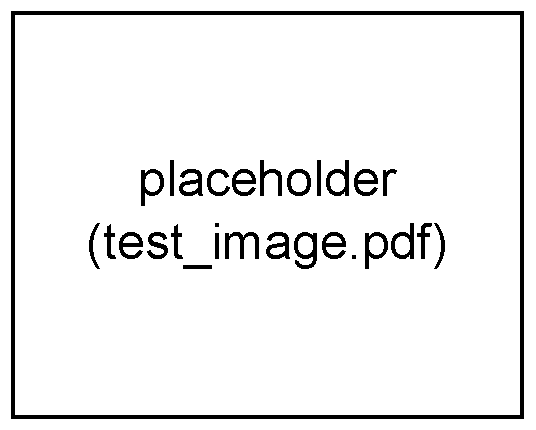
\includegraphics[width=0.8\textwidth]{\figpath/test_image.pdf}

\subsection{Critical Thinking Questions}

	\begin{enumerate}
		\item \label{ctq:ABtable} For the reaction mixture shown in Model 1, fill out the following table:
		
			\begin{table}[h]
				\centering
				\renewcommand{\arraystretch}{3}
				\begin{tabular}{|c|c|c|}
					\hline
					\textbf{Step} &  \textbf{Number of unreacted ``A'' groups} & \textbf{Number of molecules} \\\hline
					0 && \\\hline
					1 && \\\hline
					2 && \\\hline
					3 && \\\hline
					4 && \\\hline
				\end{tabular}
			\end{table}
		
		\item Explain, in a complete sentence, how the number of molecules in the mixture is related to the number of unreacted ``A'' groups.
		
		\item The number-average degree of polymerization, $N_n$, is the total number of \emph{monomers} divided by the total number of \emph{molecules}.  Remembering that we started with 8 monomers, calculate the number-average degree of polymerization for each step shown in Model 1.
		
			\begin{table}[h]
				\centering
				\renewcommand{\arraystretch}{3}
				\begin{tabular}{|c|c|c|c|c|c|}
					\hline
					\textbf{~~Step~~} &  \textbf{~~~~0~~~~} & \textbf{~~~~1~~~~} & \textbf{~~~~2~~~~} & \textbf{~~~~3~~~~} & \textbf{~~~~4~~~~} \\\hline
					$\mathbf{N_n}$ &&&&& \\\hline
				\end{tabular}
			\end{table}
		
		\item Suppose that you had initially started with 100 monomers.  Then, suppose that at some time later, you had only 8 unreacted ``A'' groups left.
		
			\begin{enumerate}
				\item How many molecules would there be in the reaction mixture at this point?
				
				\item What would the number-average degree of polymerization be at this point?
			\end{enumerate}
			
		\item More generally, suppose you started with $v_A^0$ monomers, and at some time later, you had only $v_A$ unreacted ``A'' groups left.  What would the number average-degree of polymerization be at this point, in terms of $v_A^0$ and $v_A$?
	\end{enumerate}
	
	INFORMATION: Usually, we find it more useful to work in terms of the \emph{fraction} of all ``A'' groups that have reacted, rather than the total \emph{number} of ``A'' groups that have reacted.  In step-growth polymerizations, we refer to the fraction of ``A'' groups that have reacted as the ``extent of reaction'', $p$.
	
	\begin{enumerate}
		\item If we start with $v_A^0$ ``A'' groups, how many of the ``A'' groups will have \emph{reacted} when the extent of reaction is equal to $p$?
		
		\item How many ``A'' groups are still \emph{unreacted} when the extent of reaction is equal to $p$?
		
		\item Using your answers to critical thinking questions 5, 6, and 7, derive an expression for $N_n$ in terms of $p$.
		
	\end{enumerate}

\subsection{Model 2: Polymerization of ``AA'' and ``BB''-Type Monomers}

Now, let's consider a slightly more complicated system, with two different types of monomers that each have \emph{either} two ``A'' reactive groups \emph{or} two ``B'' type reactive groups.
We call monomers with two ``A'' groups ``AA''-type monomers, and we call monomers with two ``B'' groups ``BB''-type monomers.

Suppose we start with 4 ``AA''-type monomers and 4 ``BB''-type monomers.
In this case, the evolution of the reaction mixture might look something like this:

\subsection{Critical Thinking Questions}

	\begin{enumerate}
		\item \label{ctq:AABBtable} For the reaction mixture shown in Model 2, fill out the following table:
		
			\begin{table}[!h]
				\centering
				\renewcommand{\arraystretch}{3}
				\begin{tabular}{|c|c|c|c|}
					\hline
					\textbf{Step} &  \textbf{Number of unreacted ``A'' groups} & \textbf{Number of molecules} & ~~~~$\mathbf{N_n}$~~~~\\\hline
					0 &&& \\\hline
					1 &&& \\\hline
					2 &&& \\\hline
					3 &&& \\\hline
					4 &&& \\\hline
				\end{tabular}
			\end{table}
			
		\item Compare your answers in question \ref{ctq:AABBtable} with those from question \ref{ctq:ABtable}.  What similarities and/or differences do you notice?
		
		\item Consider the following statement:
		
			\emph{``In polymerizations of AA- and BB-type monomers, we should be able to use the same expressions for calcuating $N_n$ as we did for polymerizations of AB-type monomers.''}
			
			In two or three complete sentences, briefly critique or defend this statement, making sure to explain your reasoning.
			
	\end{enumerate}

\subsection{Model 3: Polymerization of a Stoichiometrically-Imbalanced Reaction Mixture}

\subsection{Critical Thinking Questions}

	\begin{enumerate}
		\item First question?
		\item Second question?
	\end{enumerate}

\subsection{Exercises}

	After class, \textbf{read} the following sections of your textbook:
	
	\begin{enumerate}
		\item First section
		\item Second section
	\end{enumerate}
	
	Then, do the following exercises:
	
	\begin{enumerate}
		\item First exercise
		\item Second exercise
	\end{enumerate}